%%%%%%%%%%%%%%%%%%%%%%%%%%%%%%%%%%%%%%%%%%%%%%%%%%%%
%%%             Metadata                         %%%
%%%%%%%%%%%%%%%%%%%%%%%%%%%%%%%%%%%%%%%%%%%%%%%%%%%%      

\title{Grundkurs Linguistik}

\subtitle{Syntax IV: X-Bar-Theorie -- Köpfe}

\author[aMyP]{
	{\small Antonio Machicao y Priemer}
%	\\
%	{\footnotesize \url{http://www.linguistik.hu-berlin.de/staff/amyp}\\
%	\href{mailto:mapriema@hu-berlin.de}{mapriema@hu-berlin.de}}
}

\institute{Institut für deutsche Sprache und Linguistik}

%%%%%%%%%%%%%%%%%%%%%%%%%      
\date{ }
%\publishers{\textbf{6. linguistischer Methodenworkshop \\ Humboldt-Universität zu Berlin}}

%\hyphenation{nobreak}


%%%%%%%%%%%%%%%%%%%%%%%%%%%%%%%%%%%%%%%%%%%%%%%%%%%%
%%%             Preamble's End                   %%%
%%%%%%%%%%%%%%%%%%%%%%%%%%%%%%%%%%%%%%%%%%%%%%%%%%%%      


%%%%%%%%%%%%%%%%%%%%%%%%%      
\huberlintitlepage
\iftoggle{toc}{
\frame{
\begin{multicols}{2}
	\frametitle{Inhaltsverzeichnis}\tableofcontents
	%[pausesections]
\end{multicols}
	}
	}


%%%%%%%%%%%%%%%%%%%%%%%%%%%%%%%%%%
%%%%%%%%%%%%%%%%%%%%%%%%%%%%%%%%%%
%%%%%LITERATURE:


%\nocite{Altmann&Hofmann08a}
%\nocite{Altmann93a}
\nocite{Brandt&Co06a}
\nocite{Glueck05a} 
\nocite{Grewendorf&Co91a} 
\nocite{Luedeling2009a} 
%\nocite{Meibauer&Co07a}
\nocite{MuellerS13f} 
\nocite{MuellerS15b}
\nocite{Repp&Co15a} 
\nocite{Stechow&Sternefeld88a}
%\nocite{Woellstein10a}



%%%%%%%%%%%%%%%%%%%%%%%%%%%%%%%%%%
%%%%%%%%%%%%%%%%%%%%%%%%%%%%%%%%%%
\section{Einleitung}
%\frame{
%\frametitle{~}
%	\tableofcontents[currentsection]
%}

%%%%%%%%%%%%%%%%%%%%%%%%%%%%%%%%%%
\begin{frame}
\frametitle{Einleitung}

\begin{itemize}

	\item Topologisches Modell \ras nur grobe Gliederung des Satzes in 5 Felder
	\item[]	
	\item Neue feingliedrigere Modellierung \ras X-Bar-Schema
	\item[]
	\item Nicht nur für Satzpositionen, sondern auch für Relationen zwischen syntaktischen Einheiten innerhalb von Konstituenten.


\eal 
\ex[]{Peter hat gestern \alert{[den Wagen]} gekauft.}
\ex[]{\alert{[Den Wagen]} hat Peter gestern gekauft.}
\ex[]{\alert{[Den Wagen gekauft]} hat Peter gestern.} \label{ex:KonstSatz}
\ex[*]{\alert{[Den]} hat Peter gestern \alert{[Wagen]}} gekauft.
\zl

	\item Konstituenten sind nicht immer mit Satzglied gleichzusetzen \cf{\ref{ex:KonstSatz}}
	
\end{itemize}

\end{frame}


%%%%%%%%%%%%%%%%%%%%%%%%%%%%%%%%%%
\begin{frame}
\frametitle{Einleitung}

\begin{itemize}

	\item Intuitiv können wir sagen, dass die Struktur 1 grammatisch und 2 ungrammatisch ist.
	\item[]
	\eal
	\ex Klammerstruktur 1: [$_{VP}$ [$_{NP}$ [$_{Det}$Das] [$_{NP}$Brot]][$_{V}$gekauft]]
	\ex Klammerstruktur 1: [$_{??}$ [$_{Det}$Das] [$_{??}$ [$_{NP}$Brot][$_{V}$gekauft]]]
	\zl

\end{itemize}


\begin{figure}[b]
	\begin{minipage}[b]{0.05\textwidth}
	\end{minipage} 
	%
	\begin{minipage}[b]{0.40\textwidth}
	\centering
	\scriptsize{
		\begin{forest}
		sn edges,
		[Das Brot gekauft [Das Brot [Das] [Brot]][gekauft]]
		\end{forest}
		}
		\caption{Baumstruktur 1}	
  	\end{minipage}  
  	%  
	\begin{minipage}[b]{0.05\textwidth}
  	\end{minipage}
  	%         
  	\begin{minipage}[b]{0.40\textwidth}
	\centering
	\scriptsize{
		\begin{forest}
		sn edges,
		[*Das Brot gekauft [Das][Brot gekauft [Brot] [gekauft]]]
		\end{forest}
		}
		\caption{Baumstruktur 2}
  	\end{minipage}  
  	%              
	\begin{minipage}[b]{0.05\textwidth}
  	\end{minipage}
  	
\end{figure}

\begin{itemize}
	\item D.\,h., die Syntax befasst sich nicht nur mit der internen Struktur von Sätzen, sondern auch von Phrasen (machmal auch von Wörtern)
\end{itemize}
\end{frame}


%%%%%%%%%%%%%%%%%%%%%%%%%%%%%%%%%%
\begin{frame}
\frametitle{Einleitung}

\begin{itemize}

	\item Sub-Theorie der Generativen Grammatik (GG) seit den 1970er Jahren \citep{Chomsky70a, Jackendoff77a}
	\item[]	
	\item \textbf{GG:} Theoretische Richtung seit den 1950er Jahre \citep{Chomsky57a} (contra Strukturalismus)
	\item[]
	\item \textbf{Strukturalismus:}
	\begin{itemize}
		\item Empirismus (Behaviourismus)
		\item statische Theorie
		\item Beschreibungsadäquat: \textbf{Beschreibung} der in der Sprache vorkommenden Strukturen
	\end{itemize}
	
	\item \textbf{GG:}
	\begin{itemize}
		\item Rationalismus (UG)
		\item dynamische (generative) Theorie
		\item Erklärungsadäquat: \textbf{Explikation} der Kompetenz eines idealen Sprecher-Hörers
	\end{itemize}

\end{itemize}

\end{frame}


%%%%%%%%%%%%%%%%%%%%%%%%%%%%%%%%%%
\begin{frame}
\frametitle{Einleitung}

\begin{itemize}
	\item Sehr starke Tradition und Verzweigung seit den 1950er Jahren
	\item[]
	\item Sehr verschiedene Richtungen (Mainstream Generative Grammatik):
	\begin{itemize}
		\item Phrasenstrukturgrammatiken (PSG, \citet{Chomsky57a})
		\item Standardtheorie (ST, Auch Aspekte-Modell, \citet{Chomsky65a})
		\item \alert{Rektions-Bindungs-Theorie} (GB, \citet{Chomsky81a})
		\item Minimalismus (MP, \citet{Chomsky95a})
	\end{itemize}
	\item[]
	\item Daraus entstanden andere GGen:
	\begin{itemize}
		\item Generative Semantik \citep{Harris93a}
		\item Lexical-Functional Grammar (LFG)
		\item Head-driven phrase Structure Grammar (HPSG)
		\item Tree Adjoining Grammar (TAG)
		\item \dots
	\end{itemize}
\end{itemize}

\citep[s.][]{MuellerS15b}

\end{frame}


%%%%%%%%%%%%%%%%%%%%%%%%%%%%%%%%%%
%%%%%%%%%%%%%%%%%%%%%%%%%%%%%%%%%%
\subsection{GG: Grundannahmen}
%\frame{
%\frametitle{~}
%	\tableofcontents[currentsection]
%}


%%%%%%%%%%%%%%%%%%%%%%%%%%%%%%%%%%
\begin{frame}
\frametitle{GG: Grundannahmen}

\begin{itemize}
	\item Angeborene Sprachfähigkeit (UG)
	\item Prinzipien \& Parameter
	\item Strenge Modularität des Sprachsystems 
\end{itemize}

\begin{figure}
\centering

	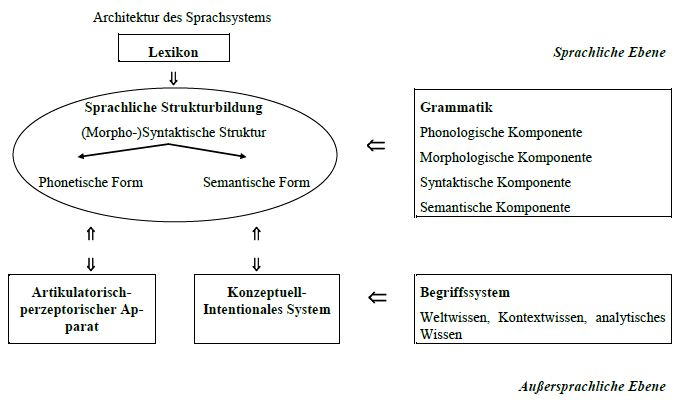
\includegraphics[scale=.3]{material/03ArchitekturSprachsystem}
	%\caption{Architektur des Sprachsystems}
\end{figure}

\end{frame}


%%%%%%%%%%%%%%%%%%%%%%%%%%%%%%%%%%
%%%%%%%%%%%%%%%%%%%%%%%%%%%%%%%%%%
\subsection{Ziele der X-Bar-Theorie}
%\frame{
%\frametitle{~}
%	\tableofcontents[currentsection]
%}


%%%%%%%%%%%%%%%%%%%%%%%%%%%%%%%%%%
\begin{frame}
\frametitle{Ziele der X-Bar-Theorie}

\begin{itemize}
	\item Explikation der syntaktischen Beziehungen zwischen einem Kopf und seinen modifizierenden (\textbf{Adjunkten}), spezifizierenden (\textbf{Spezifikatoren}), und ergänzenden (\textbf{Argumenten}) Einheiten
	\item[]
	\item Explikation endozentrischer Konstruktionen
	\item[]
	\item Bis dahin wurden Sätze als exozentrische Konstruktionen behandelt!
\end{itemize}

\begin{figure}[b]
	\begin{minipage}[b]{0.05\textwidth}
	\end{minipage} 
	%
	\begin{minipage}[b]{0.50\textwidth}
	\centering
	\footnotesize{
		\begin{forest}
		sn edges,
		[S	[NP [Stefan,triangle]]
			[VP [schreibt ein Buch, triangle]]
		]
		\end{forest}
		}
		\caption{Satz vor X-Bar-Schema}	
  	\end{minipage}  
  	%  
	\begin{minipage}[b]{0.05\textwidth}
  	\end{minipage}
  	
\end{figure}

\end{frame}


%%%%%%%%%%%%%%%%%%%%%%%%%%%%%%%%%%
%%%%%%%%%%%%%%%%%%%%%%%%%%%%%%%%%%
\section{Strukturelle Annahmen}
%\frame{
%\frametitle{~}
%	\tableofcontents[currentsection]
%}

%%%%%%%%%%%%%%%%%%%%%%%%%%%%%%%%%%
\begin{frame}
\frametitle{X-Bar: Strukturelle Annahmen}

\begin{multicols}{2}
\begin{enumerate}
	\item Alle syntaktischen Phrasen haben \textbf{den gleichen syntaktischen Aufbau}.
	\item Jede Phrase hat ein einziges, strukturell obligatorisches Element \ras \textbf{Kopf} der Phrase: \zerobar{X}, X.
	\item Zwischen Phrase und Kopf gibt es syntaktisch relevante Zwischenstufen \ras \textbf{Zwischenprojektionen}: \MyPxbar{X}, \ibar{X}.
	\item Alle Nicht-Köpfe sind \textbf{maximale Projektionen}: XP, \xxbar{X}, \iibar{X}, \maxbar{X} .
	\item Maximale Projektionen haben die gleiche Bar-Anzahl (=2).
	\item Nur Nicht-Köpfe sind optional.
\end{enumerate}
\end{multicols}

\begin{figure}[b]
	\begin{minipage}[b]{0.05\textwidth}
	\end{minipage} 
	%
	\begin{minipage}[b]{0.50\textwidth}
	\centering
	\tiny{
		\begin{forest}
		sn edges,
		[XP [YP\\Spezifikator]
			[\MyPxbar{X} [\zerobar{X}\\Kopf]
				[ZP\\Komplement]
			]
		]
		\end{forest}
		}
		\caption{X-bar Schema}	
  	\end{minipage}  
  	%  
	\begin{minipage}[b]{0.05\textwidth}
  	\end{minipage}
  	
\end{figure}

\end{frame}


%%%%%%%%%%%%%%%%%%%%%%%%%%%%%%%%%%
%%%%%%%%%%%%%%%%%%%%%%%%%%%%%%%%%%
\section{Kopf}
%\frame{
%\frametitle{~}
%	\tableofcontents[currentsection]
%}


%%%%%%%%%%%%%%%%%%%%%%%%%%%%%%%%%%
\begin{frame}
\frametitle{Kopf}

\begin{itemize}
	\item Köpfe sind bereits aus der Morphologie bekannt
\end{itemize}

\begin{figure}[b]
	\begin{minipage}[b]{0.05\textwidth}
	\end{minipage} 
	%
  	\begin{minipage}[b]{0.60\textwidth}
	\centering
	\small{
		\begin{forest}
		sn edges,
		[Autofahrer {\ras} Fahrer!
			[Auto] 
			[Fahrer]{\draw[<-,red] (.south east)--++(0em,-1.5ex)--++(+2em,0pt)
node[anchor=west,align=center]{Kopf};}
		]
		\end{forest}
		}
		\caption{Endozentrisches Kompositum}
  	\end{minipage}  
  	%              
	\begin{minipage}[b]{0.05\textwidth}
  	\end{minipage}
  	
\end{figure}

\begin{itemize}
	\item Der Kopf bestimmt die \textbf{morphosyntaktischen Eigenschaften} eines Wortes (Kasus, Numerus, Genus, Flexionsart, syntaktische Kategorie, auch semantische Aspekte, \dots )
\end{itemize}

\end{frame}


%%%%%%%%%%%%%%%%%%%%%%%%%%%%%%%%%%
\begin{frame}
\frametitle{Kopf}

\begin{block}{Kopf}
Der Kopf einer Wortgruppe/Konstituente/Phrase/Projektion ist dasjenige Element, das \textbf{die wichtigsten Eigenschaften} der Wortgruppe/Konstituente/Phrase/Projektion bestimmt. 

Gleichzeitig steuert der Kopf den \textbf{Aufbau} der Phrase, d.\,h., der Kopf verlangt die Anwesenheit bestimmter anderer Elemente in seiner Phrase.

\citep{MuellerS13f}
\end{block}

\pause

\begin{itemize}
	\item Was sind \gqq{die wichtigsten Eigenschaften}?
\end{itemize}

\end{frame}


%%%%%%%%%%%%%%%%%%%%%%%%%%%%%%%%%%
\begin{frame}
\frametitle{Kopf}

\begin{itemize}
	\item Was sind \gqq{die wichtigsten Eigenschaften}?
	\begin{itemize}
		\item Interpretation der Phrase
		\item Distribution der Phrase
		\item Morphosyntaktische Eigenschaften der Phrase
		\item Aufbau der Phrase
		
	\end{itemize}
\end{itemize}

\citep[vgl.][]{Adger04a}
\end{frame}


%%%%%%%%%%%%%%%%%%%%%%%%%%%%%%%%%%
%%%%%%%%%%%%%%%%%%%%%%%%%%%%%%%%%%
\subsection{Interpretation}
%\only<presentation>{
%\frame{
%\frametitle{~}
%	\tableofcontents[currentsection]
%}
%}

%%%%%%%%%%%%%%%%%%%%%%%%%%%%%%%%%%%
\begin{frame}
\only<presentation>{\frametitle{Interpretation}}

\begin{itemize}
	\item Sehr intuitives (aber etwas unzuverlässiges) Kriterium, v.\,a. stark theorieabhängig
	\item Durch Konstituententests wissen wir welche Wortfolgen \textbf{Konstituenten} sind.
\end{itemize}
\pause
\eal Peter kauft \alert{[das erfrischende Wasser, das ich dir letztens empfohlen habe]}.
\pause
\ex \textbf{Vorfeldtest}\\
\alert{{[}Das erfrischende Wasser, das ich dir letztens empfohlen habe]} kauft Peter. 
\pause
\ex \textbf{Fragetest}\\
\alert{{[}Was]} kauft Peter? \ras \alert{{[}Das erfrischende Wasser, das ich dir letztens empfohlen habe]}
\zl


\pause
\begin{itemize}
	\item Aber welches Wort in einer Konstituente ist der \textbf{Kopf}?
\end{itemize} 

\end{frame}


%%%%%%%%%%%%%%%%%%%%%%%%%%%%%%%%%%
\begin{frame}
\only<presentation>{\frametitle{Interpretation}}

\begin{itemize}
	\item Welches Element in der Phrase\\
	{[}Das erfrischende Wasser, das ich dir letztens empfohlen habe]\\
	steuert die Interpretation?
	\item[] \pause
	\item[\ra] \emph{Wasser} (Entität)
	\item[] \pause
	\item Welches Element in der Phrase\\
	Peter wartet \alert{[an der Ecke]}.\\
	steuert die Interpretation?
	\item[] \pause
	\item[\ra] \emph{an} (Lokation)
	\item[] \pause
	\item Welches Element in der Phrase\\
	Peter \alert{[wartet an der Ecke]}.\\
	steuert die Interpretation?
	\item[] \pause
	\item[\ra] \emph{wartet} (Handlung)

\end{itemize}

\end{frame}


%%%%%%%%%%%%%%%%%%%%%%%%%%%%%%%%%%
%%%%%%%%%%%%%%%%%%%%%%%%%%%%%%%%%%
\subsection{Distribution}
%\only<presentation>{
%\frame{
%\frametitle{~}
%	\tableofcontents[currentsection]
%}
%}

%%%%%%%%%%%%%%%%%%%%%%%%%%%%%%%%%%%
\begin{frame}
\only<presentation>{\frametitle{Distribution}}

\begin{itemize}
	\item Der Kopf bestimmt an welchen Positionen im Satz seine projizierte Phrase stehen kann:
	\begin{itemize}
		\item VPs: [\textbf{schläft}], [\textbf{kauft} den Wagen], [\textbf{schenkt} Maria die Blumen]
		\item NP: [\textbf{Peter}], [der \textbf{Wagen}], [der vermeintlich korrupte \textbf{Präsident} der FIFA]
		\item AP: [\textbf{nett}], [auf seinen Sohn \textbf{stolz}], [seiner Frau \textbf{treu}]
\end{itemize}
	\pause

\eal S \ras NP + VP
\ex[]{Peter + VP}
\ex[]{Peter + [\textbf{schläft}].}
\ex[]{Peter + [\textbf{kauft} den Wagen].}
\ex[]{Peter + [\textbf{schenkt} Maria die Blumen].}
\ex[*]{Peter + [der \textbf{Wagen}]}
\ex[*]{Peter + [seiner Frau \textbf{treu}]}
\zl
	
	
\end{itemize}

\end{frame}


%%%%%%%%%%%%%%%%%%%%%%%%%%%%%%%%%%%
\begin{frame}
\only<presentation>{\frametitle{Distribution}}

\begin{itemize}
	\item Der Kopf bestimmt an welchen Positionen im Satz seine projizierte Phrase stehen kann:
	\begin{itemize}
		\item VPs: [\textbf{schläft}], [\textbf{kauft} den Wagen], [\textbf{schenkt} Maria die Blumen]
		\item NP: [\textbf{Peter}], [der \textbf{Wagen}], [der vermeintlich korrupte \textbf{Präsident} der FIFA]
		\item AP: [\textbf{nett}], [auf seinen Sohn \textbf{stolz}], [seiner Frau \textbf{treu}]
\end{itemize}
	\pause

\eal S \ras NP + VP
\ex[]{NP + parkt an der Ecke}
\ex[]{[\textbf{Peter}] + parkt an der Ecke.}
\ex[]{[Der \textbf{Wagen}] + parkt an der Ecke.}
\ex[]{[Der vermeintlich korrupte \textbf{Präsident} der FIFA] + parkt an der Ecke.}
\ex[*]{[\textbf{Schläft}] + parkt an der Ecke.}
\ex[*]{[\textbf{Nett}] + parkt an der Ecke.}
\zl
	
	
\end{itemize}

\end{frame}


%%%%%%%%%%%%%%%%%%%%%%%%%%%%%%%%%%%
\begin{frame}
\only<presentation>{\frametitle{Distribution}}

\begin{itemize}
	\item Der Kopf bestimmt an welchen Positionen im Satz seine projizierte Phrase stehen kann:
	\begin{itemize}
		\item VPs: [\textbf{schläft}], [\textbf{kauft} den Wagen], [\textbf{schenkt} Maria die Blumen]
		\item NP: [\textbf{Peter}], [der \textbf{Wagen}], [der vermeintlich korrupte \textbf{Präsident} der FIFA]
		\item AP: [\textbf{nett}], [auf seinen Sohn \textbf{stolz}], [seiner Frau \textbf{treu}]
\end{itemize}
	\pause

\eal NP \ras Det + (AP) + N
\ex[]{Der + AP + N}
\ex[]{Der + [\textbf{nette}] + Onkel}
\ex[]{Der + [auf seinen Sohn \textbf{stolze}] + Onkel}
\ex[]{Der + [seiner Frau \textbf{treue}] + Onkel}
\ex[*]{Der + [\textbf{schläft}] + Onkel}
\ex[*]{Der + [der \textbf{Wagen}] + Onkel}
\zl
	
	
\end{itemize}

\end{frame}

%%%%%%%%%%%%%%%%%%%%%%%%%%%%%%%%%%
%%%%%%%%%%%%%%%%%%%%%%%%%%%%%%%%%%
\subsection{Morphosyntaktische Eigenschaften}
%\only<presentation>{
%\frame{
%\frametitle{~}
%	\tableofcontents[currentsection]
%}
%}

%%%%%%%%%%%%%%%%%%%%%%%%%%%%%%%%%%%
\begin{frame}
\only<presentation>{\frametitle{Morphosyntaktische Eigenschaften}}

\begin{itemize}
	\item \textbf{Kategorielle Zugehörigkeit} (Wortart \ras Phrasentyp)\\
	\ras wenn der Kopf ein \textbf{Nomen} ist, ist die gesamte Phrase eine \textbf{NP}\\
	\ras wenn der Kopf ein \textbf{Verb} ist, ist die gesamte Phrase eine \textbf{VP}
\end{itemize}

\begin{figure}[b]
	\begin{minipage}[b]{0.05\textwidth}
	\end{minipage} 
	%
	\begin{minipage}[b]{0.40\textwidth}
	\centering
	\footnotesize{
		\begin{forest}
		sn edges,
		[VP [NP [Peter,triangle]]
			[\MyPxbar{V} [NP [den Patienten,triangle]]
				[V [behandelt]]		{\draw[<-,red] (.south east)--++(0em,-1.5ex)--++(+2em,0pt)
node[anchor=west,align=center]{Kopf};}
			]
		]
		\end{forest}
		}
		\caption{VP}	
  	\end{minipage}  
  	%  
  	\pause            
	\begin{minipage}[b]{0.05\textwidth}
  	\end{minipage}
  	%         
  	\begin{minipage}[b]{0.40\textwidth}
	\centering
	\footnotesize{
		\begin{forest}
		sn edges,
		[NP [Det [Peters]]
			[\MyPxbar{N} [AP [sanfte,triangle]]
				[\MyPxbar{N} [N [Behandlung]]{\draw[<-,red] (.south west)--++(0em,-1.5ex)--++(-2em,0pt)
node[anchor=east,align=center]{Kopf};}
					[NP [des Patienten,triangle]]]]
		]
		\end{forest}
		}
		\caption{NP}
  	\end{minipage}  
  	%              
	\begin{minipage}[b]{0.05\textwidth}
  	\end{minipage}
  	
\end{figure}


\end{frame}


%%%%%%%%%%%%%%%%%%%%%%%%%%%%%%%%%%
\begin{frame}
\only<presentation>{\frametitle{Morphosyntaktische Eigenschaften}}

\begin{itemize}
	\item Der Kopf \textbf{projiziert} seine Merkmale auf die gesamte Phrase. 
\end{itemize}

\begin{tabular}{ll}
\textsc{Wortart} & \textsc{Merkmale}\\
\hline
\textbf{Verb}		& Wortart, Numerus-tragend, Person-tragend, Kasus-\\
					& determinierend, Verbform (Finitheitsmerkmale) \\
\hline
\textbf{Nomen}		& Wortart, Kasus-tragend, (Person), Numerus-tragend,\\
					& Genus-tragend, Genitiv-determinierend\\
\hline
\textbf{Adjektiv}	& Wortart, Kasus-tragend, Genus-tragend, Numerus-\\ 
					& tragend, Flexionsklasse, Kasus-determinierend\\
\hline
\textbf{Präposition}& Wortart, nicht-Kasus-tragend, nicht-Numerus-\\
					& tragend, nicht-Genus-tragend, Kasus-\\
					& determinierend\\					
\end{tabular}
\end{frame}


%%%%%%%%%%%%%%%%%%%%%%%%%%%%%%%%%%
%%%%%%%%%%%%%%%%%%%%%%%%%%%%%%%%%%
\subsection{Phrasenaufbau \ras Argumentstruktur}
%\only<presentation>{
%\frame{
%\frametitle{~}
%	\tableofcontents[currentsection]
%}
%}

%%%%%%%%%%%%%%%%%%%%%%%%%%%%%%%%%%
\begin{frame}
\frametitle{Phrasenaufbau \ras Argumentstruktur}

\begin{itemize}
	\item Auch: Valenz, Subkategorisierung
	\item[]
	\item Es wird angenommen, dass Köpfe (lexikalische Einheiten) \ua mit ihrer Argumentstruktur im \textbf{mentalen Lexikon} gespeichert sind.
	\item[]
	\item Köpfe werden aus dem Lexikon genommen und in die \textbf{syntaktische Komponente} eingefügt, wo ihre Argumentstruktur verschiedene Ebenen im X-Bar-Schema projiziert.
\end{itemize}

\end{frame}


%%%%%%%%%%%%%%%%%%%%%%%%%%%%%%%%%%
\begin{frame}
\frametitle{Phrasenaufbau \ras Argumentstruktur}

\begin{block}{Argumente und Modifikatoren}
Argumente sind die von einem Kopf (Nomen, Verb, Präposition, \dots ) verlangten Einheiten, um eine wohlgeformte Phrase zu bilden. Der Kopf bestimmt dabei die \textbf{Anzahl}, die \textbf{Form} (\zB Kasus) und die \textbf{Art} (\zB Theta-Rolle) seiner Argumente. Nicht-Argumente in einer Struktur werden \textbf{Modifikatoren} genannt. Sie werden nicht verlangt, sondern können frei hinzugefügt werden und \textbf{modifizieren} die Aussage. 
\end{block}

\end{frame}


%%%%%%%%%%%%%%%%%%%%%%%%%%%%%%%%%%%
\begin{frame}
\frametitle{Phrasenaufbau \ras Argumentstruktur}

\begin{itemize}
	\item Der Kopf bestimmt\\ 
	\textbf{welche und wieviele} Argumente \textbf{notwendig} sind, um eine wohlgeformte Phrase zu bilden.


\eal 
\ex [Peter] schläft. \hfill (1 Argument)
\ex [Peter] küsst [Maria]. \hfill (2 Argumente)
\ex [Maria] schenkt [Peter] [die Blumen]. \hfill (3 Argumente)
\zl

\pause

\eal
\ex[*]{[Peter] schläft [Maria].}
\ex[*]{[Maria] küsst [Peter] [die Blumen].}
\ex[*]{schenkt.}
\zl


\end{itemize}
\end{frame}


%%%%%%%%%%%%%%%%%%%%%%%%%%%%%%%%%%%
\begin{frame}
\only<presentation>{\frametitle{Phrasenaufbau \ras Argumentstruktur}}

\begin{itemize}
	\item Der Kopf bestimmt\\ 
	\textbf{die Form} seiner Argumente (\zB durch \textbf{Kasusrektion}).
\end{itemize}

\eal 
\ex [Der Mann]$_{\textsc{nom}}$ schläft.
\ex [Der Mann]$_{\textsc{nom}}$ küsst [den Elefanten]$_{\textsc{akk}}$.
\ex [Der Mann]$_{\textsc{nom}}$ schenkt [dem Jungen]$_{\textsc{dat}}$ [den Elefanten]$_{\textsc{akk}}$.
\ex [Der Mann]$_{\textsc{nom}}$ gedenkt [des Opfers]$_{\textsc{gen}}$.
\ex [Der Mann]$_{\textsc{nom}}$ hilft [dem Opfer]$_{\textsc{dat}}$.
\ex [Der Mann]$_{\textsc{nom}}$ wartet [auf den Jungen]$_{auf}$.
\zl

\pause

\eal
\ex[*]{[Der Mann]$_{\textsc{nom}}$ gedenkt [dem Opfer]$_{\textsc{dat}}$.}
\ex[*]{[Der Mann]$_{\textsc{nom}}$ hilft [des Opfers]$_{\textsc{gen}}$.}
\ex[*]{[Der Mann]$_{\textsc{nom}}$ wartet [den Jungen]$_{\textsc{akk}}$.}
\zl

\end{frame}


%%%%%%%%%%%%%%%%%%%%%%%%%%%%%%%%%%%
\begin{frame}
\only<presentation>{\frametitle{Phrasenaufbau \ras Argumentstruktur}}

\begin{itemize}
	\item Der Kopf bestimmt\\ 
	\textbf{die Form} seiner Argumente (\zB durch \textbf{Finitheitsrektion}).
\end{itemize}

\ea \textbf{Modalverb} verlangt Infinitiv\\
\dots dass er es \alert{kaufen$_{\textsc{inf}}$ will}
\z

\pause

\ea \textbf{\emph{haben}-Hilfsverb} verlangt Partizip II\\
\dots dass er es \alert{gekauft$_{\textsc{part}}$ hat}
\z

\pause

\ea \textbf{Modalverb} verlangt Infinitiv\\
\dots dass er es \alert{[gekauft haben]$_{\textsc{inf}}$ will}
\z

\pause

\ea \textbf{Modalverb} verlangt Infinitiv\\
\dots dass er es \alert{[gekauft haben wollen]$_{\textsc{inf}}$ muss}
\z

\pause

\ea \textbf{\emph{haben}-Hilfsverb} verlangt Partizip II\\
\dots dass er es \alert{[gekauft haben wollen müssen/gemusst]$_{\textsc{inf}}$ hat}
\z

\end{frame}


%%%%%%%%%%%%%%%%%%%%%%%%%%%%%%%%%%%
\begin{frame}
\only<presentation>{\frametitle{Phrasenaufbau \ras Argumentstruktur}}

\begin{itemize}
	\item Der Kopf bestimmt\\ 
	\textbf{die Art} wie seine Argumente interpretiert werden (Theta-Rollen, $\theta$-Rollen).

\eal 
\ex [Der Elefant]$_{\textsc{agens}}$ tötet [den Mann]$_{\textsc{patiens}}$.
\ex [Der Elefant]$_{\textsc{thema}}$ interessierte [den Mann]$_{\textsc{experiencer}}$.
\zl

\eal
\ex [Peters]$_{\textsc{agens}}$ Behandlung [des Mannes]$_{\textsc{patiens}}$
\ex [Peters]$_{\textsc{patiens}}$ Ermordung
\zl


	\item Einige Verben (\zB \obj{regnen, schneien}) vergeben ihrem Subjekt keine Theta-Rolle \ras semantisch gesehen 0-wertig

\end{itemize}

\end{frame}


%%%%%%%%%%%%%%%%%%%%%%%%%%%%%%%%%%
%%%%%%%%%%%%%%%%%%%%%%%%%%%%%%%%%%
\section{Theta-Rollen}
%\frame{
%\frametitle{~}
%	\tableofcontents[currentsection]
%}

%%%%%%%%%%%%%%%%%%%%%%%%%%%%%%%%%%
\begin{frame}
\frametitle{Theta-Rollen}

\begin{itemize}
	\item Auch: thematische / semantische Rollen, Theta-Rollen, $\theta$-Rollen
	\item[]
	\item Semantische Rolle, die ein Argument von seinem Kopf erhält
	\item[]
	\item Anzahl und Definition der Theta-Rollen \ras theorieabhängig

	\begin{itemize}
		\item \textbf{AGENS:} jemand, der die Handlung, die durch das Prädikat bezeichnet wird, willentlich anstößt/ ausführt.
		\item[]
		\item \textbf{THEMA / PATIENS:} jemand oder etwas, der oder das durch die vom Prädikat bezeichnete Handlung betroffen wird
		\item[]
		\item \textbf{EXPERIENCER:} jemand, der durch die (in der) vom Prädikat bezeichneten Handlung etwas psychisch oder physisch empfindet

	\end{itemize}

\end{itemize}

\end{frame}


%%%%%%%%%%%%%%%%%%%%%%%%%%%%%%%%%%
\begin{frame}
\frametitle{Theta-Rollen}

\begin{itemize}
	\item Anzahl und Definition der Theta-Rollen \ras theorieabhängig
	
	\begin{itemize}

		\item \textbf{ZIEL (GOAL):} die Entität, auf die die vom Prädikat ausgedrückte Handlung gerichtet ist

		\item[]
		\item \textbf{QUELLE (SOURCE):} die Entität, von der die vom Prädikat ausgedrückte Handlung ausgeht

		\item[]
		\item \textbf{ORT (LOCATION):} der Ort, an dem die vom Prädikat ausgedrückte Handlung stattfindet

		\item[]
		\item \textbf{ZEIT (TIME):} die Zeit(spanne), an der die vom Prädikat ausgedrückte Handlung stattfindet

		\item[]
		\item \textbf{POSSESSOR:} Entität, die ein Objekt besitzt		
	\end{itemize}

\end{itemize}

\end{frame}


%%%%%%%%%%%%%%%%%%%%%%%%%%%%%%%%%%
%%%%%%%%%%%%%%%%%%%%%%%%%%%%%%%%%%
\section{Subkategorisierungsrahmen}
%\frame{
%\frametitle{~}
%	\tableofcontents[currentsection]
%}

%%%%%%%%%%%%%%%%%%%%%%%%%%%%%%%%%%
\begin{frame}
\frametitle{Subkategorisierungsrahmen}

\begin{itemize}
	\item Information im Subkategorisierungsrahmen einer Kategorie:
	\item[]
	\begin{enumerate}
		\item \textbf{Anzahl} der benötigten Argumente (syntaktische Information),
		\item[]
		\item ihre \textbf{syntaktische Kategorie} (DP, PP, CP, \dots )\\
		(syntaktische Information \ras c-selektionales Merkmal oder Subkategorisierungseigenschaft),
		\item[]
		\item ihre \textbf{morphosyntaktische Realisierung} (\zB Kasus) (morphologische Information),
		\item[]
		\item ihre \textbf{$\theta$-Rolle} (semantische Information),
		\item[]
		\item \textbf{weitere semantische Eigenschaften}, \zB das Objekt vom Verb \obj{trinken} muss \gqq{flüssig} sein (semantische Information \ras s-selektionales Merkmal oder 	Selektionsbeschränkung).
	\end{enumerate}
	
\end{itemize}

\end{frame}


%%%%%%%%%%%%%%%%%%%%%%%%%%%%%%%%%%
\begin{frame}
\frametitle{Subkategorisierungsrahmen}

\begin{itemize}

	\item Die Information der Argumentstruktur im Subkategorisierungsrahmen:
	
	\ea lesen: DP$_{\textsc{nom,ag}}$ (DP)$_{\textsc{akk,th}}$ $\underline{\qquad}$
	\z
	
	\item[] \textbf{=} \obj{lesen} ist subkategorisiert für zwei Argumente, die beide syntaktisch NPn/DPn sind. Eine der NPn/DPn ist obligatorisch, wird im Nominativ realisiert und trägt die $\theta$-Rolle Agens, z.B. \obj{Uta} in \obj {Uta liest ein Buch}. Die andere NP/DP ist fakultativ, wird im Akkusativ realisiert und trägt die $\theta$-Rolle Thema (\zB \obj{ein Buch} in \obj{Uta liest ein Buch}).

	\ea schenken: DP$_{\textsc{nom,ag}}$ DP$_{\textsc{dat,ziel}}$  DP$_{\textsc{akk,th}}$ $\underline{\qquad}$ 
	\z
		
\end{itemize}

\end{frame}


%%%%%%%%%%%%%%%%%%%%%%%%%%%%%%%%%%
%%%%%%%%%%%%%%%%%%%%%%%%%%%%%%%%%%
\section{Modifikatoren (vs. Argumente)}
%\frame{
%\frametitle{~}
%	\tableofcontents[currentsection]
%}

%%%%%%%%%%%%%%%%%%%%%%%%%%%%%%%%%%
\begin{frame}
\frametitle{Modifikatoren vs. Argumente}

\textbf{Modifikatoren} sind vom Kopf weitgehend unabhängig in Bezug auf\dots

\begin{itemize}
	\item \textbf{Anzahl}

\eal 
\ex Maria schläft \alert{[heute] [im Zimmer] [unruhig]}.
\ex Maria küsst Peter \alert{[heute] [im Zimmer] [unruhig]}.
\ex Maria schenkt Peter die Blumen \alert{[heute] [im Zimmer] [unruhig]}.
\zl

	\begin{itemize}
		\item Modifikatoren sind \textbf{immer fakultativ}!
		\item Argumente können \textbf{obligatorisch} oder \textbf{fakultativ} sein (sie werden dann \gqq{mitverstanden}! \ras existentielle Interpretation)
		
		\eal 
		\ex Maria schläft \alert{[heute] [im Zimmer]}.
		\ex Maria schläft \alert{[im Zimmer]}. 
		\zl
		
		\eal 
		\ex Peter isst \alert{[eine Schokolade]}.
		\ex Peter isst. 
		\zl
		
	\end{itemize}

\end{itemize}

\end{frame}


%%%%%%%%%%%%%%%%%%%%%%%%%%%%%%%%%%
\begin{frame}
\frametitle{Modifikatoren vs. Argumente}

\textbf{Modifikatoren} sind vom Kopf weitgehend unabhängig in Bezug auf\dots

\begin{itemize}
	
	\item \textbf{Form}
\eal
\ex Maria schläft \alert{[heute]$_{AdvP}$ [im Zimmer]$_{PP}$, [obwohl die Heizung nicht funktioniert]$_{CP}$}.
\ex Maria küsst Peter \alert{[heute]$_{AdvP}$ [im Zimmer]$_{PP}$, [obwohl die Heizung nicht funktioniert]$_{CP}$}.
\ex Maria schenkt Peter die Blumen \alert{[heute]$_{AdvP}$ [im Zimmer]$_{PP}$, [obwohl die Heizung nicht funktioniert]$_{CP}$}.
\zl

\end{itemize}

\end{frame}


%%%%%%%%%%%%%%%%%%%%%%%%%%%%%%%%%%
\begin{frame}
\frametitle{Modifikatoren vs. Argumente}

\textbf{Modifikatoren} (syntaktisch: Adjunkte) sind vom Kopf weitgehend unabhängig in Bezug auf\dots

\begin{itemize}
	\item \textbf{Art}

\eal 
\ex Der Ingenieur sprengte \alert{[die Brücke]$_{\textsc{pat}}$}. 
\ex Der Ingenieur sah \alert{[die Brücke]$_{\textsc{th}}$}. 
\ex Der Ingenieur verließ \alert{[die Brücke]$_{\textsc{quelle}}$}.
\zl

	\begin{itemize}
		\item Modifikatoren der gleichen Art sind \textbf{iterierbar}!
		\item Argumente der gleichen Art sind \textbf{nicht iterierbar}!
		
		\eal 
		\ex[]{Maria schläft \alert{[heute]$_{\textsc{zeit}}$ [am frühen Morgen]$_{\textsc{zeit}}$}.}
		\ex[*]{Peter isst \alert{[eine Schokolade]$_{\textsc{th}}$ [einen Kuchen]$_{\textsc{th}}$}.}
		\zl

		
	\end{itemize}

\end{itemize}

\end{frame}


%%%%%%%%%%%%%%%%%%%%%%%%%%%%%%%%%%
%%%%%%%%%%%%%%%%%%%%%%%%%%%%%%%%%%
\section{Übungen}
%\frame{
%\frametitle{~}
%	\tableofcontents[currentsection]
%}

%%%%%%%%%%%%%%%%%%%%%%%%%%%%%%%%%%
\begin{frame}
\frametitle{Übungen}

\begin{itemize}

	\item Bestimmen Sie den Kopf der folgenden Phrase und begründen Sie Ihre Entscheidung:
	
		\ea Es geht um [\textbf{wirklich von dieser Sache überzeugte und engagierte junge Schüler, die sich dennoch über das übliche und akzeptable Ausmaß hinaus daneben benommen haben}].
		\z
	

	\pause
	\item[\ra] Nominalphrase/Substantivgruppe\\
	Kopf: Nomen \emph{Schüler}\\
	da Schüler sowohl die Genus-, Kasus- und Numerus-Eigenschaften der Gesamtphrase bestimmt, ihre mögliche interne Modifikation (\zB \emph{junge}, \emph{engagierte}), wie auch wesentliche ihrer semantischen Eigenschaften 
	
\end{itemize}

\end{frame}


%%%%%%%%%%%%%%%%%%%%%%%%%%%%%%%%%%
\begin{frame}
\frametitle{Übungen}

\begin{itemize}

	\item Geben Sie die Argumentstruktur (in dem bekannten Format) und einen Beispielsatz der von Ihnen angegebenen AS für die folgenden Wörter an:\\
	übergeben, stolz, regnen, glauben, Frage, wissen, donnern, scheinen, mit, erschrecken, ängstigen, fürchten, Banane, Tatsache, warten, Angst, wohnen, bewohnen, auf, malen, krank, bemalen, fragen

\end{itemize}

\end{frame}
